%&preamble
% Save static part at preamble.tex and use command:
% xelatex -ini -shell-escape -job-name="preamble" "&xelatex preamble.tex\dump"
% to produce preamble.fmt

% Only for xelatex and lualatex. It provides an automatic and unified interface to feature-rich AAT and OpenType fonts.
% https://ctan.org/pkg/fontspec
\usepackage{fontspec}
\setmainfont{DejaVu Serif}
\renewcommand{\contentsname}{Περιεχόμενα}
\renewcommand{\listfigurename}{Λίστα Σχημάτων}
\renewcommand{\figurename}{Σχήμα}
\renewcommand{\lstlistingname}{Καταχώρηση}
\renewcommand{\lstlistlistingname}{List of \lstlistingname s}

\title{4η Εργασία στα Παράλληλα και Διανεμημένα Συστήματα\\Pagerank}
\author{Ορέστης Φλώρος-Μαλιβίτσης, 7796\\
  Χαμζάς Κωσταντίνος, 7798\\
  Τομέας Ηλεκτρονικής,\\
  Τμήμα Ηλ. Μηχανικών / Μηχανικών ΗΥ,\\
  Αριστοτέλειο Πανεπιστήμιο Θεσσαλονίκης}
\titlepic{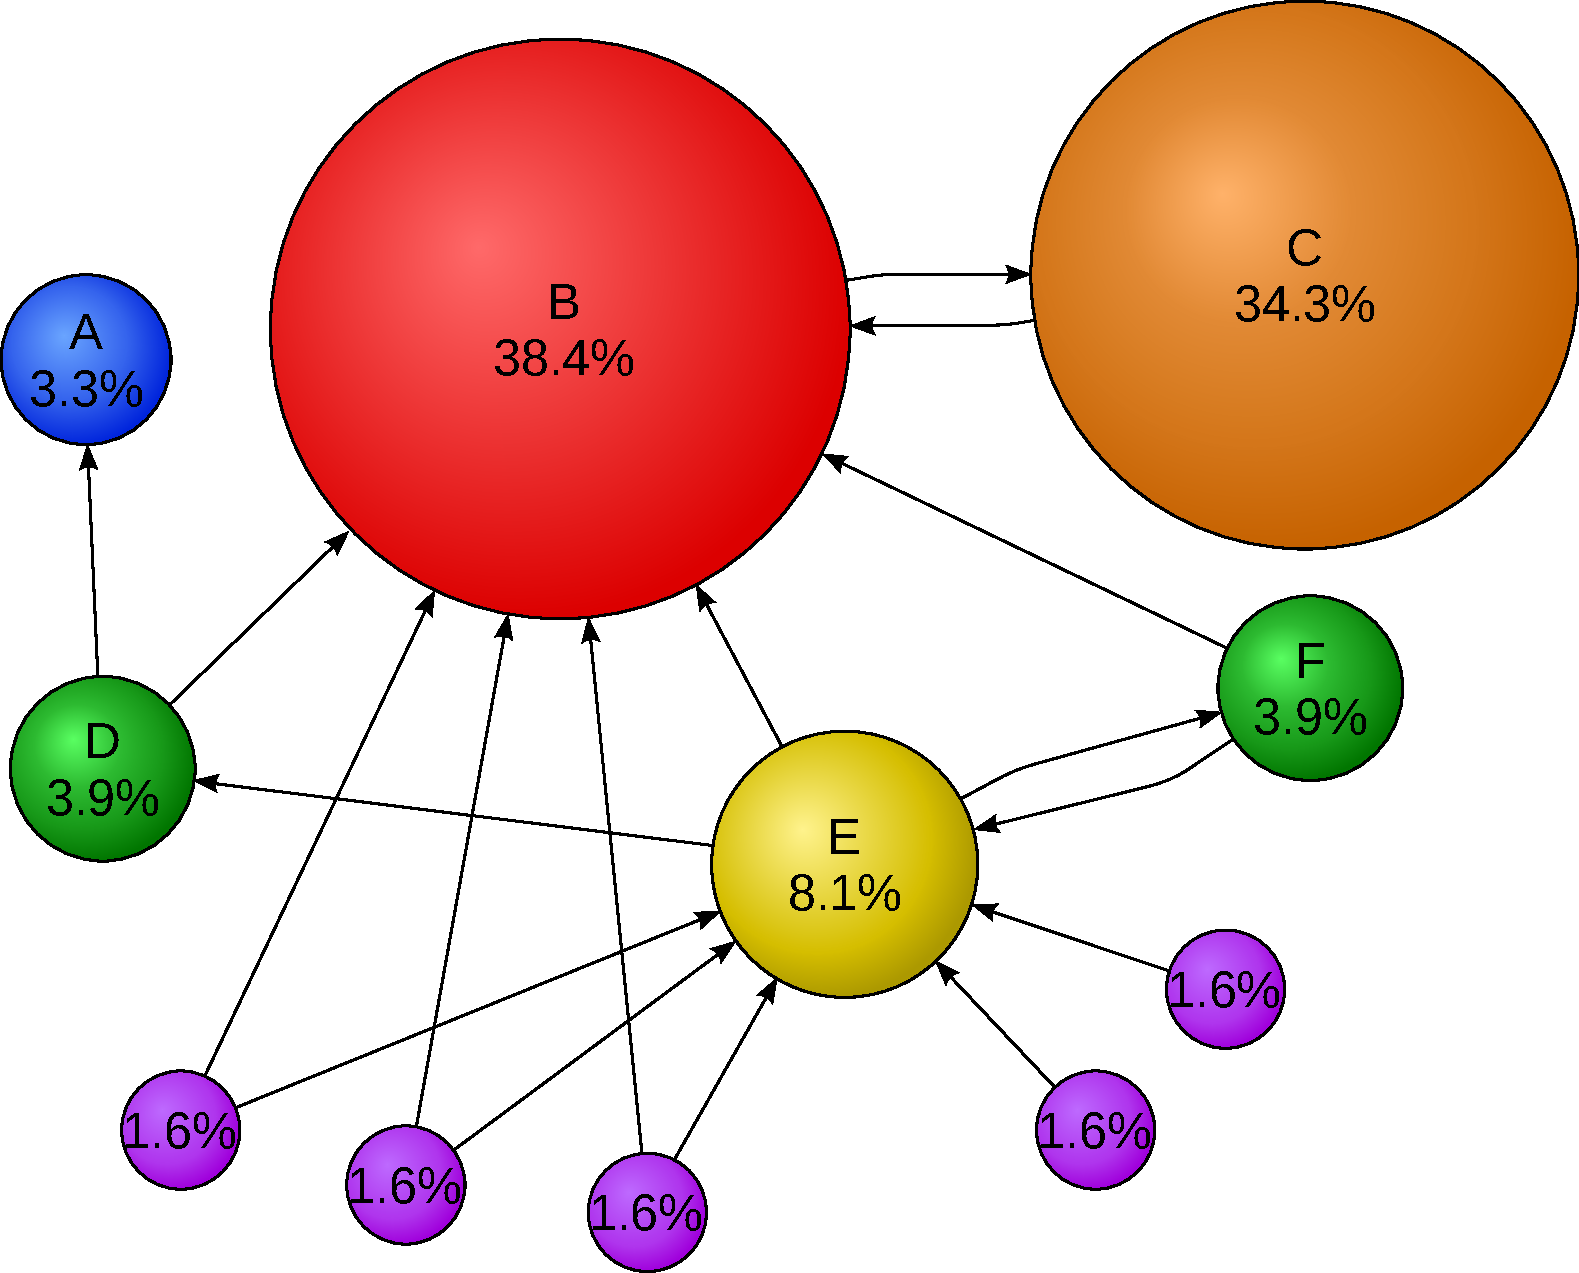
\includegraphics[width=0.85\textwidth]{pagerank-cover.pdf}}
\begin{document}
\maketitle
\tableofcontents
%\listoffigures
\newpage

% Δομή του Project
\chapter*{Δομή του Project} \label{project-structure}

\begin{description}
	\item[doc/] Φάκελος με τα *.tex αρχεία για την παραγωγή της αναφοράς.
	\item[doc/plot/] Φάκελος με τα αρχεία των γραφημάτων.
	\item[page-rank.pdf] Η εκφώνηση.
	\item[main.c] Ο κώδικας του προγράμματος σε c.
	\item[matlab/] Φάκελος με τα scripts σε MATLAB.
	\item[report.pdf] Αυτή η αναφορά.
	\item[run\_data.py] Script σε python3 για την παραγωγή δεδομένων και τον έλεγχό τους.
\end{description}

\noindent Για build τρέχουμε:
\begin{lstlisting}[language=bash, caption={build commands}, escapechar=$]
mkdir bin
cd bin
cmake ..
make
\end{lstlisting}

\chapter{Εισαγωγή}
Στη Συγκεκριμένη εργασία μας ζητείται να υλοποιήσουμε παράλληλα τον αλγόριθμο Page-rank σε ένα κατευθυνόμενο γράφο .
Ο αλγόριθμος αυτός χρησιμοποιείται για την 'μέτρηση' 
της σχετικής σημαντικότητας του κάθε κόμβου μέσα σε αυτόν τον γράφο  .
Αν θεωρήσουμε ως κατευθυνόμενο γράφο ένα κομμάτι του διαδικτύου,όπου οι κόμβο αντιστοιχούν σε ιστοσελίδες
και οι ακμές σε συνδέσεις(link) από την μία ιστοσελίδα στην άλλη τότε 
Ο αλγόριθμος είναι ο ακόλουθος:\\
  \begin{equation*}
  \bold {P^{t+1}_i = d \sum_{j \in B_i} P^t_j  \frac{a_{ij}}{ \sum_{k \in B_j} {a_{jk}} } + (1-d)E_i}
  \end{equation*}
  
  Όπου :
\begin{enumerate}
	\item $P^{t+1}_i$ η πιθανότητα να βρεθεί στον κόμβο i την χρονική στιγμή t+1
	\item $P^t_j$η πιθανότητα να βρεθεί στον κόμβο j την χρονική στιγμή t
	\item $a_{ij}$  δυαδική μεταβλητή που δείχνει την ύπαρξη σύνδεσης από τον κόμβο i στον j
	\item $B_i$ τα σύνολα των κόμβων με τους οποίους συνδέεται ο i
	\item $E_i$ η πιθανότητα ο χρήστης να βρεθεί στον κόμβο i μέσω μιας τυχαίας αναζήτησης.
	\item $\sum_{k \in B_j}$ o βαθμός συνδεσιμότητας του κόμβου j.
	\item $d$ παράγοντας που καθορίζει την σημασία του κάθε όρου της εξίσωσης  
\end{enumerate}

Μετά το πέρας ενός ικανού αριθμού βημάτων 
διάνυσμα P σταθεροποιείται αντανακλώντας τις πιθανότητες κάποιος χρήστης να βρίσκεται στην κάθε  ιστοσελίδα
κάποια μελλοντική στιγμή .(Εννοείται αν οι επιλογές του είναι μόνο οι ιστοσελίδες που έχουμε συμπεριλάβει.)
 
  Στην  εικόνα εξωφύλλου φαίνεται το  αποτέλεσμα που παράγει ένας τέτοιος αλγόριθμος. 
  
\chapter{Υλοποίηση σε C}

Το αρχείο main.c περιέχει την \lstinline!main()! συνάρτηση του προγράμματος
και την συνάρτηση \lstinline!calculate_pagerank()!
που είναι η κυρίως ρουτίνα για τον υπολογισμό του διανύσματος $P$.

Το αρχείο io.c περιέχει συναρτήσεις σχετικά με την επικοινωνία του προγράμματος με τον χρήστη.

\section{io.c}
Από την \lstinline!print_usage()!, οι επιλογές του προγράμματος είναι:

\begin{verbatim}
usage: ./assignment_4 [options]

	-h, --help: This help.
	-n, --nodes-file=FILENAME: File to use for input graph. Default is nodes.txt
	-t, --nthreads=NUM: Number of threads used to run pagerank.
	-f, --custom-f: Binary file to use for initial P. Default is uniform distribution.
	-e, --custom-e: Binary file to use for initial E. Default is uniform distribution.
	-s, --smart-split: Split work between threads based on workload, not nodes.
\end{verbatim}

Η συνάρτηση \lstinline!read_from_file()! ανοίγει το αρχείο που προσδιορίζεται από την επιλογή \lstinline!--nodes-file=! και
διαβάζει τον γράφο για στον οποίο θα εκτελεσθεί ο pagerank.
Γίνεται η υπόθεση ότι το αρχείο είναι απλό text file όπου τα σχόλια αρχίζουν με '\#' και υπάρχουν
2 ακέραιοι ανά γραμμή. Ο δεύτερος συμβολίζει τον node στον οποίο καταλήγει ο πρώτος.

Η συνάρτηση \lstinline!print_gen()! αποθηκεύει το αποτέλεσμα $P$ σε ένα binary file.
Η \lstinline!save_res()! αποθηκεύει πληροφορίες όπως χρόνος εκτέλεσης, αριθμός threads, αριθμός γενεών και μέγεθος.

Η συνάρτηση \lstinline!init_prob()! αρχικοποιεί τις τιμές των $P$, $E$.
Αν δεν δοθεί αρχείο από το οποίο μπορούν να διαβαστούν οι αρχικές τιμές τους, χρησιμοποιείται ομοιόμορφη κατανομή.

Η συνάρτηση \lstinline!argument_praser()! επεξεργάζεται τα ορίσματα που δίνονται στο πρόγραμμα.

\section{main.c}

Η συνάρτηση \lstinline!split_work()! χρησιμοποιείται για να αρχικοποιήσει τα ορίσματα των threads και να μοιράσει την δουλειά μεταξύ τους.
Αν είναι ενεργή η επιλογή \lstinline!--smart-split!, ο διαμοιρασμός των nodes στα threads γίνεται με βάση των αριθμό των inbound links του καθενός.
Αλλιώς, μοιράζονται ομοιόμορφα με το κάθε thread να παίρνει $\frac{N}{nthreads}$ nodes.

Η συνάρτηση \lstinline!calculate_pagerank()! πραγματοποιεί τους υπολογισμούς για το pa\-ge\-rank του $P$.
Η συνάρτηση έχει υλοποιηθεί έτσι ώστε να έχει ίδιο αποτέλεσμα με το script του MATLAB.

Στην μεταβλητή \lstinline!prob_type link_prob! υπολογίζεται η πιθανότητα από την σύνδεση μέσω κάποιου άλλου κόμβου.
Το \lstinline!node_id n_inbound[i]! είναι ο αριθμός των εισερχόμενων κόμβων στον κόμβο \lstinline!i!
ενώ ο \lstinline!node_id n_inbound[j]! ο αριθμός των εξερχόμενων από τον j.
Η εντολή \lstinline!const node_id j = L[i][x];! θέτει στην \lstinline!j! το x-οστό εισερχόμενο κόμβο στον i-οστό κόμβο.
\begin{lstlisting}[caption={υπολογισμός link\_prob}, escapechar=$]
prob_type link_prob = 0;
for (node_id x = 0; x < n_inbound[i]; x++) {
    const node_id j = L[i][x];
    link_prob += P[j] / n_outbound[j];
}
link_prob += constant_add;
\end{lstlisting}
Το \lstinline!constant_add! είναι η \hyperref[line:c_eq_0]{ποσότητα} που προστίθεται και στη συνάρτηση pagerankpow.m της MATLAB.
Υπολογίζεται σε κάθε επανάληψη από ένα thread και είναι κοινό για όλα τα threads.
Ο υπολογισμός γίνεται από την \hyperref[lst:calculate_const_add]{calculate\_const\_add()}.
Ο πίνακας \lstinline!node_id *no_outbounds! κρατάει τα στοιχεία χωρίς εξερχόμενους κόμβους.
\begin{lstlisting}[language=matlab, caption={το constant\_add στο pagerankpow.m}, escapechar=$]
if c(j) == 0
	x = x + z(j)/n;$\label{line:c_eq_0}$
else
	x(L{j}) = x(L{j}) + z(j)/c(j);
end
\end{lstlisting}

\begin{lstlisting}[caption={υπολογισμός const\_add}, escapechar=$, label={lst:calculate_const_add}]
float calculate_const_add(void) {
    // calculate the constant for links without outbound links.
    float res = 0.0f;
    for (node_id x = 0; x < size_no_out; x++) {
        const node_id j = no_outbounds[x];
        res += P[j];
    }
    res /= (prob_type) N;
    return res;
}
\end{lstlisting}

Αν χρησιμοποιείται ομοιόμορφη κατανομή για το $E$ προϋπολογίζεται η τιμή $(1-d) \cdot E$ ως:
\lstinline!const prob_type const_E = (1 - D) / (prob_type) N;!.
Αλλιώς, χρησιμοποιείται το array \lstinline!prob_type *E!.

Για τον τερματισμό των threads χρησιμοποιείται ο πίνακας \lstinline!static bool *local_terminate_flag!.
Κάθε thread ελέγχει μία \hyperref[lst:local_terminate]{συνθήκη συνέχειας} για κάθε στοιχείο του \lstinline!P!.
\begin{lstlisting}[caption={έλεγχο συνέχειας ανά thread}, escapechar=$, label={lst:local_terminate}]
P_new[i] = D * link_prob + (args->custom_E ? (1 - D) * E[i] : const_E);
if (local_terminate_flag[tid]) {
    if (fabsf(P_new[i] - P[i]) > MAX_ERROR) {
        local_terminate_flag[tid] = 0;
    }
}
\end{lstlisting}

Στο τέλος κάθε επανάληψης ένα thread αναλαμβάνει να:
\begin{itemize}
	\item κάνει \hyperref[line:swap-P-P_new]{swap} τους pointers \lstinline!P! και \lstinline!P_new! 
	\item \hyperref[line:global-check-terminate]{ελέγξει} αν οι συνθήκες συνέχειας είναι \lstinline!false! για κάθε thread
	\item \hyperref[line:call-calculate_const_add]{καλέσει} την \lstinline!calculate_const_add()!
\end{itemize}
\begin{lstlisting}[caption={swap P, P\_new και έλεγχος τερματισμού.}, escapechar=$, label={lst:gen_barrier}]
const int res = pthread_barrier_wait(&barrier);
if (res == PTHREAD_BARRIER_SERIAL_THREAD) {
    // swap P_new with P.$\label{line:swap-P-P_new}$
    prob_type *tmp;
    tmp = P;
    P = P_new;
    P_new = tmp;

    running = false;$\label{line:global-check-terminate}$
    for (unsigned int i = 0; i < nthreads; i++) {
        if (!local_terminate_flag[i]) {
            running = true;
            break;
        }
    }
    if (running) {
        constant_add = calculate_const_add();$\label{line:call-calculate_const_add}$
    }
}

pthread_barrier_wait(&barrier);
if (!running) break;
\end{lstlisting}
Τα υπόλοιπα threads περιμένουν για την επόμενη γενιά ή τερματίζονται αν \lstinline!running == false!.
\chapter{Αποτελέσματα}
Σε αυτό το κομμάτι παρουσιάζονται όλα τα πειραματικά αποτελέσματα.
\section{Έλεγχος ορθότητας}
Εδώ φαίνονται τα τελικά αποτελέσματα (rankings) που προέκυψαν από την εφαρμογή του αλγορίθμου σε 2 διαφορετικούς γράφους.

Το πρώτο προέκυψε με την χρήση της συνάρτηση surfer.m στη σελίδα \href{http://stackoverflow.com/}{stackoverflow.com}.
O γράφος που δημιουργήθηκε από το stackoveflow φαίνεται στο
\hyperref[fig:stackGraph]{\figurename{} \ref{fig:stackGraph}}
\begin{figure}[h]
	\centerline{\includegraphics[width=0.6\textwidth]{stackGraph.pdf}}
	\caption{Ο γράφος συνδέσεων}
	\label{fig:stackGraph}
\end{figure}
 
Τα αποτελέσματα για τη MATLAB και τη C φαίνονται στο \hyperref[fig:stackres]{\figurename{} \ref{fig:stackres}}
\begin{figure}[h]
	\centerline{\includegraphics[width=0.85\textwidth]{stackres.pdf}}
	\caption{Αποτελέσματα για stackoverflow}
	\label{fig:stackres}
\end{figure}
 
Βλέπουμε ότι τα αποτελέσματα μεταξύ των 2 υλοποιήσεων ταυτίζονται σε πολύ μεγάλο βαθμό.
Επίσης, σε σχέση με το
\hyperref[fig:stackGraph]{\figurename{} \ref{fig:stackGraph}}
μπορούμε να επιβεβαιώσουμε  εποπτικά την ορθότητα των αποτελέσματά μας
παρατηρώντας ότι οι μεγαλύτερες πιθανότητες εμφανίζονται στους κόμβους 40 και 90
οι οποίοι  σύμφωνα με το 
\hyperref[fig:stackGraph]{\figurename{} \ref{fig:stackGraph}}
έχουν τα περισσότερα links προς αυτούς (κάθετος άξονας).
Επίσης, ο αριθμός των επαναλήψεων που χρειάστηκε για να συγκλίνει το $P$ ήταν 40.
Ο κάνονας που θέσαμε ήταν να μην υπάρχει μεταβολή μεγαλύτερη του $10^{-6}$ σε σχέση με το προηγούμενο $P$ για οποιονδήποτε κόμβο.
Η μεγάλη συνδεσιμότητα του γράφου
(\href{https://en.wikipedia.org/wiki/Clustering_coefficient#Global_clustering_coefficient}{average clustering coefficient} 0.518)
δικαιολογεί το σχετικά μεγάλο αυτό νούμερο καθώς οι μεταβολές θα ήταν πολύ πυκνές και συχνά αλληλοαναιρούμενες.

\newpage

Για το δεύτερο αποτέλεσμα χρησιμοποιήθηκε γράφος όπου προέρχεται από αυτό το
\href{http://snap.stanford.edu/data/soc-Slashdot0811.html}{link} 
και περιέχει ένα δίκτυο από το
\href{http://slashdot.org/}{http://slashdot.org/}
και φαίνεται στο
\hyperref[fig:slashGraph]{\figurename{} \ref{fig:slashGraph}}
\begin{figure}[h!]
	\centering
	\subfloat[]{\includegraphics[width=0.5\textwidth]{slash.png}}
	\subfloat[]{\includegraphics[width=0.5\textwidth]{slashGraphDet.pdf}}
	\caption{O γράφος συνδέσεων με μία λεπτομέρεια στα αριστερά}
	\label{fig:slashGraph}
\end{figure}

Ο γράφος δεν είναι τόσο πυκνός όσο φαίνεται.
Από μία λεπτομέρεια στην πάνω αριστερά γωνία διαφαίνεται ότι είναι αρκετά αραιός,
έχει
\href{https://en.wikipedia.org/wiki/Clustering_coefficient#Global_clustering_coefficient}{average clustering coefficient} 0.055499.

Το ranking που προκύπτει για αυτό το δίκτυο φαίνεται στο
\hyperref[fig:slackres]{\figurename{} \ref{fig:slackres}}.
\begin{figure}[h!t]
	\centering
	\includegraphics[width=0.9\textwidth]{slashdot.png}
	\caption{Αποτελέσματα για slashdot}
	\label{fig:slackres}
\end{figure}
Επιβεβαιώνουμε την ορθότητα των αποτελεσμάτων μας με το ίδιο σκεπτικό όπως στην προηγούμενη περίπτωση.
Βλέπουμε λοιπόν ότι η παράλληλη υλοποίηση δουλεύει σωστά και για πολύ μεγαλύτερο αριθμό κόμβων.
Τέλος, πρέπει να σημειώσουμε ότι τα βήματα που χρειάστηκαν για την σύγκλιση ήταν μόλις 19.
Θα περίμενε κανείς ότι ένας μεγαλύτερος γράφος με τόσο μεγάλη ασυμμετρία θα χρειαζόταν περισσότερα βήματα για να συγκλίνει σε σχέση με το γράφο του stackoveflow.
Το γεγονός όμως ότι είναι πολύ πιο αραιός τον κάνει να συγκλίνει στο τελικό διάνυσμα πολύ πιο γρήγορα.
\clearpage
\section{Χρόνος εκτέλεσης}
Οι γράφοι που χρησιμοποιήθηκαν βρίσκονται στα ακόλουθα link:\\
\begin{enumerate} 
	\item \href{https://snap.stanford.edu/data/wiki-Vote.html}{Wiki-Vote}.
	\item \href{https://snap.stanford.edu/data/email-EuAll.html}{email-EuAll}.
	\item\href{https://snap.stanford.edu/data/web-BerkStan.html}{web-BerkStan}.
	\item\href{https://snap.stanford.edu/data/web-NotreDame.html}{web-NotreDame}.
	\item\href{https://snap.stanford.edu/data/web-Google.html}{web-Google}.
	\item\href{https://snap.stanford.edu/data/soc-pokec.html}{soc-pokec}.
\end{enumerate}
%TODO: link dropbox με τα παντα
%TODO: graphs με coeff

\clearpage
\section{Σύγκλιση γενεών}


\end{document}
